\documentclass{llncs}

% you'll probably need this if you want to include images
\usepackage{graphicx} 
\usepackage{amssymb}
\usepackage[dvipsnames]{xcolor}
\usepackage{amsmath}
\usepackage{amsfonts}
\usepackage{proof}
\usepackage{url,hyperref}

\newtheorem{theorem}{Theorem}
\newtheorem{definition}{Definition}
\newtheorem{corollary}[theorem]{Corollary}
\newtheorem{conjecture}[theorem]{Conjecture}
\newtheorem{lemma}[theorem]{Lemma}
\newtheorem{example}{Example}
\newtheorem{exercise}{Exercise}
\newcommand{\code}[1]{\texttt{#1}}
\newcommand{\eat}[1]{}
\newcommand{\hook}{\supset}
\date{}

\definecolor{PurpleViridis}{HTML}{440154}
\definecolor{GreenViridis}{HTML}{55C667}
\definecolor{BlueViridis}{HTML}{33638D}

\begin{document}

\author{Venetsia Krasteva}
\title{Pilot's Assistance System for an Aircraft}
\institute{Edinburgh Napier University  \\
    SET10112/SET10412 Formal Approaches to Software Engineering}

\maketitle

\begin{abstract}
This report describes the implementation of a pilots assistance system for an aircraft using the Ada-SPARK specifications and bodies for the system.The system implements all the features described in the specification. There are two types of extensions added to the program to extend its complexity and aid demonstration. All functions and procedures pass Gold Level of SPARK which means it is a Platinum level program. 
\end{abstract}

\section{Introduction}\label{plane}
The aim of this report is to describe the implementation of the developed pilot's assistance system and to demonstrate that the procedures and functions are formally verified. Following OO programming design principle, the  plane is broken down into classes, each class is a particular part of the plane that stores their states in a record which are then used in plane to implement main features that are used in main:

\begin{itemize}
\item \textbf{plane} - Uses other classes features to develop a working program.
\item \textbf{door} - Controls all doors in plane.
\item \textbf{altitude} - Controls altitude of plane and landing gear.
\item \textbf{fuel} - Controls fuel and fuel warning light.
\item \textbf{speed} - Controls the speed.
\item \textbf{main} - Used to aid demonstration of working program.
\end{itemize}

For the development of the Pilot's System, the programming ADA was used in compliance with SPARK for formal proof of the functionality of the program. 

\section{Controller Structure}
This is another section
\begin{itemize}
\item \textbf{\underline{door}} - defines the doors that can be found on the plane. This package contains four different kinds of doors ({\textbf{Cock pit}}, {\textbf{extenal}}, {\textbf{toilet}} and {\textbf{cabin doors}}). {\textbf{Cock pit door}} and {\textbf{external doors}} are used with the record {\textbf{\textit{Door}}}. {\textbf{Toilet doors}} and {\textbf{cabin doors}} are combined wit the record {\textbf{Passenger Utilities Door}}. Each record is used in order to determine the \textbf{status } \textit{Closed/Open} and \textbf{lock status} \textit{Locked/Unlocked} and when they are \textit{Closed} and \textit{Locked}, the global variables of type boolean {\textbf{Is\_Ct\_Ext\_Lock\_Close}}) and {\textbf{Util\_Doors\_Locked\_Closed}} will be \textit{True}, which will be used in package \textbf{plane}.
\item \textbf{\underline{fuel}} - implements the fuel system that tracks the {\textbf{levels of fuel}} \textit{(0,...,45)}. Given how much fuel we have, our {\textbf{\textit{PlaneFuelTank}}} record stores {\textbf{the status}}  \textit{Low} $($fuelLevels $<$ $15$)$/$\textit{Sufficient} $($fuelLevels $\geqslant$ 15$)$ of fuel and whether or not the {\textbf{warning fuel light}} is \textit{On/Off}. The record is used in \textbf{\underline{plane}} package in order to work with other elements.
\item \textbf{\underline{speed}} - used to track the current {\textbf{speed}} \textit{$($0,...,10$)$} of the aircraft and depending on the speed, a {\textbf{mode}} \textit{(standby} $($speed $=$ 0$)$, \textit{speeding} $($speed $<$ 6$)$, \textit{takingofflanding} $($speed = 6$)$, \textit{normal} (speed $>6$) is assigned to the record {\textbf{\textit{Speedometer}}}.
\item \textbf{\underline{altitude}} - implements the altitude system that track the {\textbf{altitude}} \textit{(0,...,30)} of the plane and assigns a {\textbf{mode}} \textit{(standby} $($altitude $=$ 0$)$, \textit{takingofflanding} $($altitude $<$ 20$)$, \textit{normal} (altitude $\geqslant$ 20)) to it. In addition, depending on the {\textbf{altitude}}, whether {\textbf{lowering the landing gear}}  can be \textit{fine (<10)/notfine($\geqslant$10}. These states are added to a record {\textbf{\textit{Altitudometer}}}.
\item \textbf{\underline{plane}} - The elements stored as records from \textbf{\underline{door}}, \textbf{\underline{fuel}}, \textbf{\underline{speed}} and \textbf{\underline{altitude}} are used to build the plane. \textbf{\underline{Plane}} package itself has a {\textbf{plane mode}} (\textit{standBy}, \textit{takeoffLanding}, \textit{normal}) variable that is assigned depending on what {\textbf{altitude}} and {\textbf{speed mode}} are. Depending form package whether or not it is \textit{fine}/\textit{notfine}, the {\textbf{landing gear}} element in {\textbf{plane}} can be \textit{Lowered}/\textit{Unlowered}. The {\textbf{engine}}, {\textbf{towing}} and {\textbf{warning limit lights}} elements can be \textit{On}/\textit{Off}.
\end{itemize}

The system is using two global variables in order to determine if the doors are locked and these values are then used in plane in order to provide the desired functionality of the program. 
Separating the code into packages allowed a faster development, better understandably and maintainability of the code itself as each packages describes an element of the plane and they all have functions and procedures. 
The records are used in the plane package in combined with other features in order to bring the desired functionality of the code. 
The main package uses the same analogy as the plane (we use the records and the two global variables) in other to create an automatic demonstration of the plane from turning on the engine to towing it (end result) and then it repeats itself.

\section{Descriptions of procedures and functions}
Pre-conditions are used to define what the variables must be initially to satisfy the post-condition wichi is the outcome of our procedure. Invariant Functions need to be true all the time. When a variable is in it means that it is read or initialised and when it is an out it means that the the value will be changed. 
\subsection{Door}
The door package is crucial to the system as without it the doors may be open and unlocked during flight which would be dangerous for eveyone attending the flight. Usind SPARK we are verifying the functionality and the procedures correctness in order to not have the case where the External Doors and Cockpit door is unlocked and open. 
This package only includes procedures to Open/Close and Unlock/Lock the doors. In addition, Is\_Cockpit\_External\_Locked\_Closed and Util\_Doors\_Locked\_Closed (included as an extension) are assigned the value of True whenever the doors are closed and locked. These global variables play an essential role in the plane package as without them the plane would not be able to take off. The system uses two types of records because whenever the plane is flying in normal mode the utility doors will be unlocked.
The records {\textbf{\textit{Doors}}} and {\textbf{\textit{Passenger\_Utility\_Doors}}} both have components {\textbf{status}} and {\textbf{lock}} so variables defining {\textbf{Cockpit\_Door}}, {\textbf{External\_Doors}}, {\textbf{Toilet\_Doors}} and {\textbf{Cabin\_Doors}} are created which are then used in procedures to ensure the desired functionality.  
\begin{itemize}
\item \textbf{close\_External\_Cockpit\_Doors} -This procedure closes the doors  suing the the Global variables {\textbf{Cockpit\_Door}, \textbf{External\_Doors}} as In\_Out because we read them and write to them. The post-condition is Cockpit\_Door.status = Closed and External\_Doors.status = Closed and a pre-condition is not needed because we do not need to specify anything in order to satisfy the post-condition. 
\item \textbf{Lock\_All\_Doors} - This procedure locks  the Cockpit\_Door and  External\_Doors where as pre-condition we are expecting the doors to already be Closed. In order to ensure nothing has changed while executing the procedure it is specified in the post-condition that doors need to be closed and locked. 
\item \textbf{Is\_Lock\_External\_Cockpit} -  Ensures that both doors are closed and locked so as Global Variables we need as input Cockpit\_Door and External\_Doors in order to read their state and as an output variable we need {\textbf{Is\_Ct\_Ext\_Lock\_Close}} as we will change its value depending on the status of the doors. 
\end{itemize}
\subsection{Fuel}
Fuel package implements everything going on with the fuel in the plane. It has three types: fuel\_Status (Low/Sufficient), warn\_Sign (on/off) and Fuel\_Levels with range from 0,...,45. Depending on what fuel level is the plane the states are stored in a record Plane\_Fuel\_Tank with status (of type fuel\_Status) and warning (of type warn\_Sign). This package contains extensions discussed in the extensions section. The procedures and function:
\begin{itemize}
\item \textbf{Fuel\_Invariant} - Takes into account the record Plane\_Fuel\_Tank and states that the warning light cannot be off when the status of fuel is Low. This Invariant is added to all procedures in the package to ensure it is \textbf{never} the case where the fuel is Low and warning light is off.
\item \textbf{Fuel\_Level\_Invariant} - ensures fuel never goes out of range as it ensures it is never lower than the first value or bigger than last value. 
\item \textbf{Low\_Sufficient\_Fuel\_Level} - This procedure takes as input the record Plane\_Fuel\_Tank and checks the fuel level of the plane and assigns (output) the status of fuel and warning of the Plane\_Fuel\_Tank.  The pre-condition is the Invariants and current level of fuel to be  $<$15 or $\geqslant$ 15.  The post-condition is the Invariants. This procedure makes sure that the warning will display Low/Sufficient fuel no matter the state the plane is in (extension to "Once in flight, the system will warn of low fuel.".
\end{itemize}
\subsection{Speed}
This package controls the speed (range of 0,...,10) of the plane and and assigns it to a mode in the record Speedometer which has the component current\_Speed\_Type (standby, speeding, takeoff\_landing, normal). This package contains extensions discussed in the extensions section.
\begin{itemize}
\item \textbf{Speed\_Invariant} - This invariant makes sure the speed does not go out of range as it ensures it is never lower than the first value or bigger than last value. 
\item \textbf{Assign\_Speed\_Mode} -  The record is passes as an in out variable because we need to initialize the variable and assign a new value to it. This procedure uses the Speed Invariant as Pre- and Post-Condition. The procedure checks what is the current speed of the plane and assigns it into a mode. This procedure is used within extensions of system.
\end{itemize}
\subsection{Altitude}
The package Altitude tracks the current altitude of range 0,...,30 and assigns it to an Altitude\_Type (standby,takeoff\_Landing, normal). Depending on the current\_altitude, lowering the landing gear can fine/notFine. The type of the altitude whether or not it is fine to lower the landing gear or not is all stored in the record Altitudometer. The package contains extensions discussed in the extensions section.
\begin{itemize}
\item \textbf{Altitude\_Invariant} - This invariant makes sure the altitude does not go out of range as it ensures it is never lower than the first value or bigger than last value. 
\item \textbf{Assign\_Altutude\_Mode} - This procedure has the Altitudometer as in out variable and checks the current altitude is and depending on its value it is assigned a mode in order to be used in plane package. As Pre- and Post-Condition we use the Altitude\_Invariant.
\item \textbf{Check\_Altitude\_For\_Landing\_Gear} - This procedure will tell the pilot if it is fine to lower the landing gear or not depending on the current\_altitude. As a pre- and post-condition we have the Altitude\_Invariant. In addition, if current\_altitude $>$ 10 then the lowering the landing gear cannot be fine is added to the post-condition .  
\end{itemize}
\subsection{Plane}
Plane package implements the whole functionality of the program using all the packages above in order to create and meet desired functionality of system. \\Plane has three global variables Ready\_TakeOff, Landing and DoorsOK of type Boolean. Package  has the types: Plane\_Mode (stand\_by, takeoff\_Landing, normal), Landing\_Gear (lowered, unlowered), Engine (on,off), Towing (on,off), Warning\_Limit\_Light (on,off) and separate variables were created in order to represent the structure of the plane:
\begin{itemize}
\item \textbf{curr\_Plane\_mode} (of type Plane\_Mode) - represents the current mode the plane is on depending on the altitude and speed.
\item \textbf{curr\_land\_gear} (of type Landing\_Gear) - represents whether or not the lading gear is lowered or unlowered. 
\item \textbf{curr\_Engine} (of type Engine) - represents if the plane is powered up or not.
\item \textbf{curr\_tow} (of type Towing) - represents if the plane is in towing mode or not. 
\item \textbf{curr\_Fuel} (of type Plane\_Fuel\_Tank) -  lets the pilot know if the plane has sufficicent/low fuel and if warning light is on/off.
\item \textbf{curr\_speed} (of type Speedometer) - represent the current speed mode that is calculated form speed package. 
\item \textbf{curr\_altitude} (of type Altitudometer) - represent the current altitude mode and whether or not it is fine/notFine to lower the landing gear.
\item \textbf{curr\_warning\_limit}(of type Warning\_Limit\_Light) - represent if warning light is on when current plane mode, altitude mode and speed more are not the same. 
\end{itemize}
The functions (some are extensions) and procedures are as listed bellow: 
\begin{itemize}
\item \textbf{Engine\_Tow\_Invariant} - function that returns Boolean to make sure that Engine is off when Towing is on.
\item \textbf{Engine\_Invariant} - if the plane is powered on and if plane mode is takeoff\_landing or normal then the towing cannot be on. 
\item \textbf{TakeOff\_Doors} - As input Is\_Ct\_Ext\_Lock\_Close, Util\_Doors\_Locked\_Closed  and curr\_Plane\_Mode and Doors\_OK as output. It checks if the plane is in stand\_By mode and if doors are locked and if yes then Doors\_OK = True otherwise False. The post-condition ( Doors\_OK = True or Doors\_OK = False) holds after the procedure is executed so no pre-condition is needed.
\item \textbf{TakeOff\_Fuel} - This procedure will not allow the plane mode to be changed to takekeoff\_Landing (out Plane\_Mode) because  it checks if there is a sufficient level of fuel (in Plane\_Fuel\_Tank) before switching to taking off mode, if low on fuel the plane will stay in stand\_By mode. This procedure does not need a pre-condition as it the post-condition holds when procedure is done executing.
\item \textbf{Landing\_Gear\_Enabler} - This procedure has curr\_Plane\_Mode, curr\_altitude as an in variables because our procedure checks what the current state of the plane in and checks if it is fine to lower the landing gear and have curr\_land\_gear as an in out because we need to have it initialized and we will change the value. The post condition makes sure that curr\_Plane\_Mode does not change when procedure is executed and curr\_land\_gear can be either lowered or unlowered. The pre-condition only needs to be curr\_Plane\_Mode = takeoff\_Landing because that is when the lowering gear can be modified only.  
\item \textbf{Towing\_Mode} -  curr\_Engine is passed to the procedure as an out variable because we do not need to know what state is it in as we will only modify it while curr\_tow will be an in variable because we need to know whether it is on/off in order to turn off the engine. The post-condition is only the Engine\_Tow\_Invariant because we have to make sure when towing is on the engine is off in all times. Because we need the plane mode to be stand\_By, we include it in the pre-condition combined with the Engine\_Tow\_Invariant.
\item \textbf{Warning\_Limit\_Light\_On\_OFF} - This procedure will turn the warning limit light on when speed mode, altitude mode and plane mode are not in the same mode. As in variables we need to have curr\_Plane\_mode,  curr\_speed, curr\_altitude and as an out variable curr\_warning\_limit because we will changed in based on the in variables. Here the post-condition makes sure that curr\_Plane\_mode,  curr\_speed, curr\_altitude are in the same mode(such as = normal) but because the types are initialised in every package separately with a different naming we include all of the possible combinations or curr\_warning\_limit = on. No pre-condition is needed here.
\item \textbf{Normal\_Flight\_Speed\_Altitude} - This funciton checks the altitude mode, speed mode, and the plane mode if they are normal. As Contract\_Cases we included that the doors need to be closed with the Invariant Fly\_Mode\_Doors and specified that if they are all normal then the function returns true, otherwise False  
\end{itemize}
\section{Mark  Proof of Consistency}
Every procedure and function within the application are formally verified using the SPARK proof system and manual calculation of pre-conditions depending on what the procedure is doing.
An important procedure is the locking function of the doors because we have to make sure that they are closed initially and then lock them otherwise it will be dangerous for passengers and crew member to be on board of the plane while flying. \\
That is why in this case we will demonstrate that the proof obligations as satisfied.
In order to do that we first need to replace the new variables in our post-condition with the old variables.\\
\[
\begin{array}{cl}
(c_D.status = cl \wedge ext_D.status = cl)\hook\{c_D.lock := Locked; ext_D.lock = Locked\}\\
((c_D.locked = Locked \wedge c_D.status = cl)\wedge(ext_D.lock = Locked \wedge ext_D.status = cl) \\
 \\
=  (c_D.status = cl \wedge ext_D.status = cl)\hook((Locked = Locked \wedge c_D.status = cl)
\\\wedge
\\(Locked = Locked \wedge ext_D.status = cl) \\
 \\
=  (c_D.status = cl \wedge ext_D.status = cl)\hook((\top \wedge c_D.status = cl) \wedge (\top \wedge ext_D.status = cl)
\\
=  (c_D.status = cl\wedge ext_D.status = cl)\hook(c_D.status = cl) \wedge (ext_D.status = cl)   &  Since T\wedge P = P
\end{array}
\\
\]
Now we can use Sequent Calculus to prove that the pre-condition indeed implies the post-condition using a derivation tree. \\
\[
\infer[R\hook]{\Rightarrow (c_D.st = cl \wedge ext_D.st= cl)\hook(c_D.st = cl \wedge ext_D.st = cl)}
	{\infer[L\wedge]{c_D.st = cl \wedge ext_D.st = cl \Rightarrow c_D.st = cl \wedge ext_D.st = cl} {\infer[R\wedge]{c_D.st = cl, ext_D.st = cl \Rightarrow c_D.st = cl \wedge ext_D.st = cl}
	{\infer[Ax]{c_D.st = cl, ext_D.st = cl \Rightarrow  c_D.st = cl} & \infer [Ax]{c_D.st = cl, ext_D.st = cl \Rightarrow ext_D.st = cl }}}}
\]
\section{Extensions}
In the program there are a lot of extensions that enable the program to execute a working demonstration from powering on the plane to shutting down and switching to towing mode. 
Extension which introduce new complexity to the formal part of the system:
\subsection{Fuel}
\begin{itemize}
\item \textbf{Add\_Fuel} - takes into account the Plane\_Fuel\_Tank and whether is is bellow ($<$15) or above ($\geqslant$ 15) it changes the status and warning sign. As post-condition we have  that the function must return the changed fuel level or the old one. Because our procedure has calculations in it we need to make sure it does not go out of range so because the procedure adds one to the old fuel level we make sure it is $\geqslant$ to 0 and it is it it $<$ 45.
\item \textbf{Burn\_Fuel} - Plane\_Fuel\_Tank is an in out variable because we need to have it initialised and changed depending on the fuel\_Level. The post-condition  includes the Invariants and makes sure that the fuel is decreasing or does not change. In the pre-condition we include the invariants and make sure that when decreased the fuel\_Level is not out of range. 
\end{itemize}
\subsection{Door}
Here the extensions added are functions such as unlocking doors and extra passenger utility doors which will be unlocked during normal flight mode. When the Passenger\_Utility\_Doors are locked and closed the Global variable Util\_Doors\_Locked\_Closed accessible throughout the program is changed to True. 
\subsection{Altitude}
\begin{itemize}
\item \textbf{Accelerate\_Altitude} - makes sure that the altitude increases (post-condition) or when max reached it stays the same until decreased. current\_altitude and the record Altitudometer are passes as in out variables because they need to be read and changed on execution of the procedure. The pre-condition includes the Invariant of Altitude and makes sure it is not bigger than the last Altitude. 
\item \textbf{Decrease\_Altitude} - this procedure makes sure that the Altitude decreases and or stays the same when min has been reached. The current\_altitude and the record Altitudometer are passes as in out variables because they are read and changed. As pre-condition the Invariant is added and it makes sure that the current\_altitude that will get changed is not bigger that the max. 
\end{itemize}
\subsection{Speed}
\begin{itemize}
\item \textbf{Accelerate\_Speed} - This procedure is equivalent to Add\_Fuel and Accelerate\_Altitude. The only changes are that it increases the speed.
\item \textbf{Decrease\_Speed} - This procedure is equivalent to Burn\_Fuel and Decrease\_Altitude. The only changes are that it decreases the speed.
\end{itemize}
\subsection{Plane}
\begin{itemize}
\item \textbf{Flight\_Speed\_Altitude} - this is an extension to the program where it assigns the modes to the plane according to the speed and altitude mode. 
\item \textbf{Ready\_To\_TakeOff} - As global variables we need to have Is\_Ct\_Ext\_Lock\_Close and  Util\_Doors\_Locked\_Closed as input and  Doors\_OK and Ready\_TakeOff as output. This procedure executes TakeOff\_Doors and TakeOff\_Fuel (in Plane\_Fuel\_Tank) and depending on Doors\_OK and fuel status (will change plane mode to take off if Sufficient (out Plane\_Mode), Ready\_TakeOff will be assigned True/False. We do not need a post-condition as we are only checking if the plane is ready to take off, but curr\_Plane\_Mode has to be stand\_By to satisfy the procedure upon execution. 
\item {Power\_On\_Mode/Power\_Off\_Mode} -  These procedures allow the plane to turn on and off. Power\_On\_Mode has post-condition ensuring that the plane mode is stand\_By and the engine is on and because of our else statement we include curr\_Engine = off and curr\_Plane\_mode = stand\_By (ensure the mode of the plane has not changed) and Engine\_Invariant, Engine\_Tow\_Invariant (make sure towing mode is off). As pre-conditions we include the Engine\_Invariant, Engine\_Tow\_Invariant and plane mode must be stand\_By when powering on.  Power\_Off\_Mode turns the plane off and we need to make sure that plane is in stand\_By mode when executing (pre-condition) this procedure and when execution is done (post-condition). The Engine\_Invariant is included to make sure the plane is on when not it stand\_By mode or towing is on. 
\end{itemize}
The extension aiding demonstrating the correctness of the formal part of the system:
This extension is located in the main package and uses all procedures including extension procedures to aid the demonstration of the plane. The demonstration is build as an automatic plane that turns on, checks doors (if open and unlocked then close and lock) and fuel (if low then add fuel). Then the plane speeds up until it reaches a certain speed and it start to increase altitude until normal modes are reached. During flight mode the plane unlocks passenger utility doors so the passengers can use - toilet and cabin doors, and before landing mode it locks them again. During landing it decreases speed and when a certain limit is reached the altitude starts to decrease. The modes are synchronised throughout the program. As soon as it lands it it unlocks the passenger utility doors and then the external doors  giving airport members time to safely attach the stairs so passenger can leave the plane. Then the plane switched engine off and towing mode is enabled. 
\\
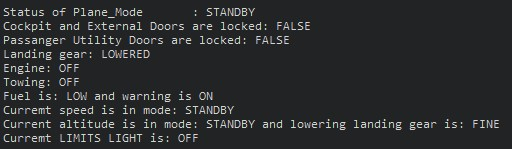
\includegraphics{planeimg.jpg}

\\
\section{Conclusion}

\begin{quote} A quote
\end{quote}




\end{document}